% ---- wrapper to allow tabular below tikzpicture in standalone ----
\begin{minipage}{18.5cm}

\begin{center}
\small\textbf{Unit balls $B_1(0)$ for five metrics on $\mathbb{R}^2$}
\medskip

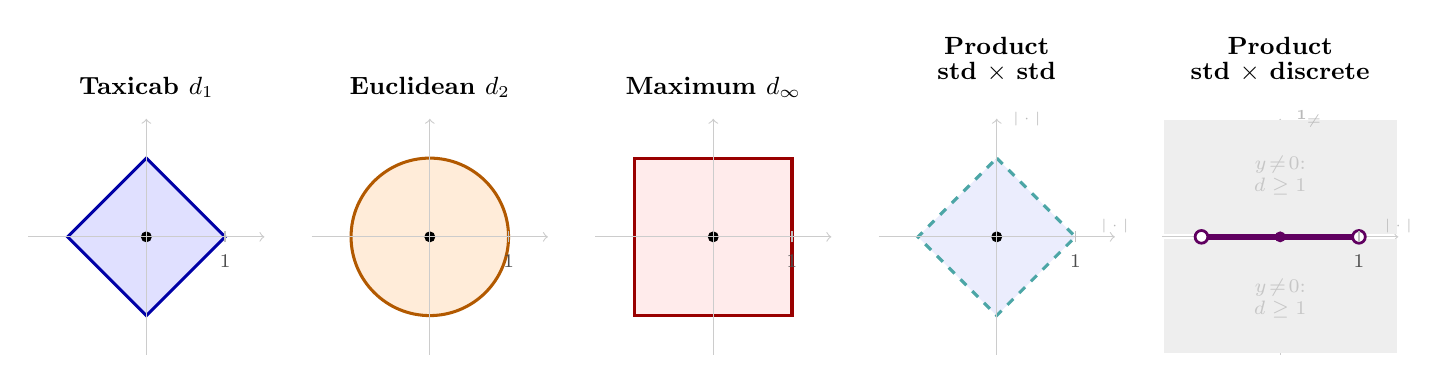
\begin{tikzpicture}[
  dot/.style={circle,fill,inner sep=1.4pt},
  lbl/.style={font=\small},
  sublbl/.style={font=\scriptsize,text=gray!60!black},
]
\def\dx{3.6}
\def\s{1.0}

% ----- Panel 1: d1 taxicab -----
\begin{scope}[shift={(0,0)}]
  \fill[blue!12]   (0,\s)--(\s,0)--(0,-\s)--(-\s,0)--cycle;
  \draw[blue!65!black,line width=1.1pt] (0,\s)--(\s,0)--(0,-\s)--(-\s,0)--cycle;
  \node[dot] at (0,0) {};
  \draw[gray!40,->] (-1.5,0)--(1.5,0);
  \draw[gray!40,->] (0,-1.5)--(0,1.5);
  \draw[gray!50,line width=0.5pt] (\s,-2pt)--(\s,2pt);
  \node[sublbl,anchor=north] at (\s,-3pt) {$1$};
  \node[lbl,font=\small\bfseries,anchor=south] at (0,1.65) {Taxicab $d_1$};
\end{scope}

% ----- Panel 2: d2 Euclidean -----
\begin{scope}[shift={(\dx,0)}]
  \fill[orange!15] (0,0) circle (\s);
  \draw[orange!70!black,line width=1.1pt] (0,0) circle (\s);
  \node[dot] at (0,0) {};
  \draw[gray!40,->] (-1.5,0)--(1.5,0);
  \draw[gray!40,->] (0,-1.5)--(0,1.5);
  \draw[gray!50,line width=0.5pt] (\s,-2pt)--(\s,2pt);
  \node[sublbl,anchor=north] at (\s,-3pt) {$1$};
  \node[lbl,font=\small\bfseries,anchor=south] at (0,1.65) {Euclidean $d_2$};
\end{scope}

% ----- Panel 3: d_inf max/square -----
\begin{scope}[shift={(2*\dx,0)}]
  \fill[red!8]  (-\s,-\s) rectangle (\s,\s);
  \draw[red!60!black,line width=1.1pt] (-\s,-\s) rectangle (\s,\s);
  \node[dot] at (0,0) {};
  \draw[gray!40,->] (-1.5,0)--(1.5,0);
  \draw[gray!40,->] (0,-1.5)--(0,1.5);
  \draw[gray!50,line width=0.5pt] (\s,-2pt)--(\s,2pt);
  \node[sublbl,anchor=north] at (\s,-3pt) {$1$};
  \node[lbl,font=\small\bfseries,anchor=south] at (0,1.65) {Maximum $d_\infty$};
\end{scope}

% ----- Panel 4: product std x std -----
\begin{scope}[shift={(3*\dx,0)}]
  \fill[green!10!blue!8] (0,\s)--(\s,0)--(0,-\s)--(-\s,0)--cycle;
  \draw[green!50!blue!70,line width=1.1pt,dashed]
    (0,\s)--(\s,0)--(0,-\s)--(-\s,0)--cycle;
  \node[dot] at (0,0) {};
  \draw[gray!40,->] (-1.5,0)--(1.5,0);
  \draw[gray!40,->] (0,-1.5)--(0,1.5);
  \draw[gray!50,line width=0.5pt] (\s,-2pt)--(\s,2pt);
  \node[sublbl,anchor=north] at (\s,-3pt) {$1$};
  \node[sublbl,text=gray!55,anchor=south] at (1.5,-0.08) {\tiny$|\cdot|$};
  \node[sublbl,text=gray!55,anchor=west,rotate=0] at (0.08,1.5) {\tiny$|\cdot|$};
  \node[lbl,font=\small\bfseries,anchor=south,align=center] at (0,1.85)
    {Product\\[-2pt]std $\times$ std};
\end{scope}

% ----- Panel 5: product std x discrete -----
\begin{scope}[shift={(4*\dx,0)}]
  \draw[gray!40,->] (-1.5,0)--(1.5,0);
  \draw[gray!40,->] (0,-1.5)--(0,1.5);
  % forbidden band shading
  \fill[gray!13] (-1.48, 0.03) rectangle (1.48, 1.48);
  \fill[gray!13] (-1.48,-1.48) rectangle (1.48,-0.03);
  \node[sublbl,align=center,text=gray!45] at (0, 0.78) {$y\!\neq\!0$:\\$d\ge 1$};
  \node[sublbl,align=center,text=gray!45] at (0,-0.78) {$y\!\neq\!0$:\\$d\ge 1$};
  % unit ball segment
  \draw[violet!75!black,line width=2.4pt] (-\s,0)--(\s,0);
  \draw[violet!75!black,fill=white,line width=1.0pt] (-\s,0) circle (2.3pt);
  \draw[violet!75!black,fill=white,line width=1.0pt] ( \s,0) circle (2.3pt);
  \node[dot,fill=violet!75!black] at (0,0) {};
  \draw[gray!50,line width=0.5pt] (\s,-2pt)--(\s,2pt);
  \node[sublbl,anchor=north] at (\s,-3pt) {$1$};
  \node[sublbl,text=gray!55,anchor=south] at (1.5,-0.08) {\tiny$|\cdot|$};
  \node[sublbl,text=gray!55,anchor=west] at (0.08,1.5) {\tiny$\mathbf{1}_{\neq}$};
  \node[lbl,font=\small\bfseries,anchor=south,align=center] at (0,1.85)
    {Product\\[-2pt]std $\times$ discrete};
\end{scope}

\end{tikzpicture}

\smallskip
\begin{tabular}{@{} l l l @{}}
\toprule
\textbf{Panel} & \textbf{Metric} & \textbf{Unit ball $B_1(0)$} \\
\midrule
Taxicab $d_1$
  & $d_1 = |x_1-y_1|+|x_2-y_2|$
  & Diamond (square rotated $45°$) \\
Euclidean $d_2$
  & $d_2 = \sqrt{(x_1-y_1)^2+(x_2-y_2)^2}$
  & Disc \\
Maximum $d_\infty$
  & $d_\infty = \max(|x_1-y_1|,\,|x_2-y_2|)$
  & Square (axis-aligned) \\
Product std $\times$ std
  & $d = |x_1-x_2|+|y_1-y_2|$
  & Diamond — same as $d_1$ \\
Product std $\times$ discrete
  & $d = |x_1-x_2|+\mathbf{1}_{y_1\neq y_2}$
  & Open segment $\{(x,0):|x|<1\}$ only \\
\bottomrule
\end{tabular}

\smallskip
{\scriptsize\color{gray!60!black}
Panels 1--3: all three standard metrics are equivalent (same open sets, same convergent sequences). \quad
Panel 4: product of two standard metrics recovers $d_1$. \quad
Panel 5: standard $\times$ discrete --- unit ball collapses to a 1-D segment; every off-axis point is at distance $\ge 1$.}

\end{center}
\end{minipage}